As problem \eqref{problem:seperated_problem} and \eqref{problem:shared_problem} are multi-objective optimization problems, we can obtain
the Pareto optimal front by varying the regularization parameter $\rho$, which is
capable of revealing the tradeoff relationship between different objectives, i.e., 
probing power at target and WSR. Figure \ref{fig:tradeoff_single_fully} shows the Pareto optimal fronts 
of the RIS-aided and normal DFRC systems.

\begin{figure}[h]
    \centering
    \subfigure[Separated deployment: $\varepsilon = 0$]{
        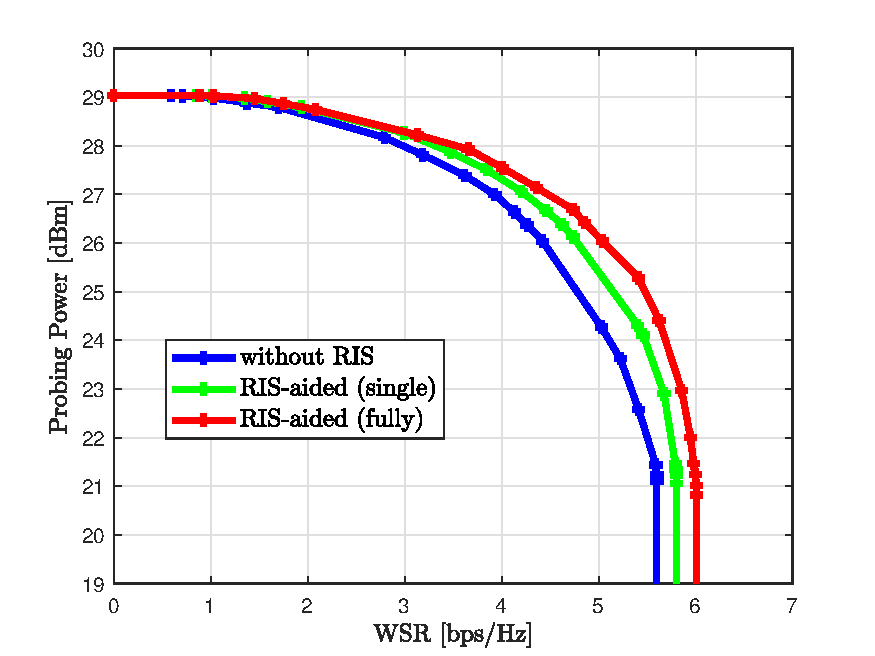
\includegraphics[width=0.475\textwidth]{tradeoff_single_fully_a.pdf}
        \label{fig:tradeoff_single_fully_a}
    }
    \subfigure[Separated deployment: $\varepsilon = 1000$]{
    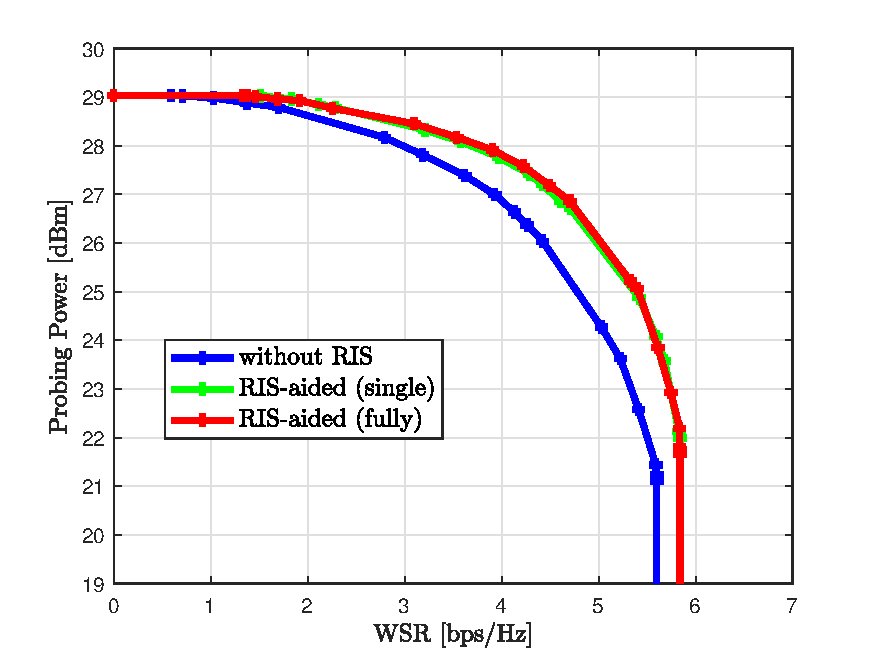
\includegraphics[width=0.475\textwidth]{tradeoff_single_fully_b.pdf}
        \label{fig:tradeoff_single_fully_b}
    }
    \subfigure[Shared deployment: $\varepsilon = 0$]{
        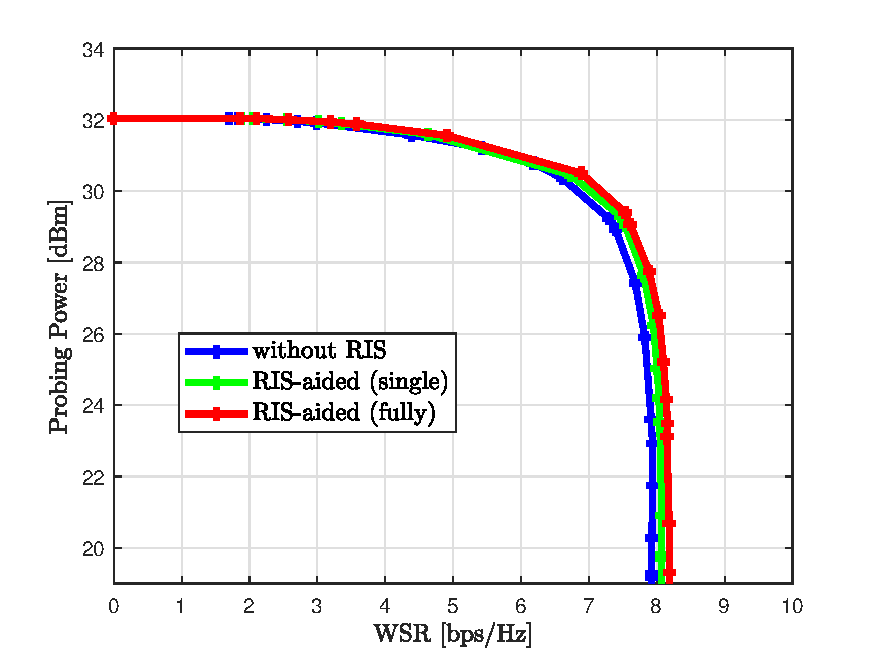
\includegraphics[width=0.475\textwidth]{tradeoff_single_fully_c.pdf}
        \label{fig:tradeoff_single_fully_c}
    }
    \subfigure[Shared deployment: $\varepsilon = 1000$]{
    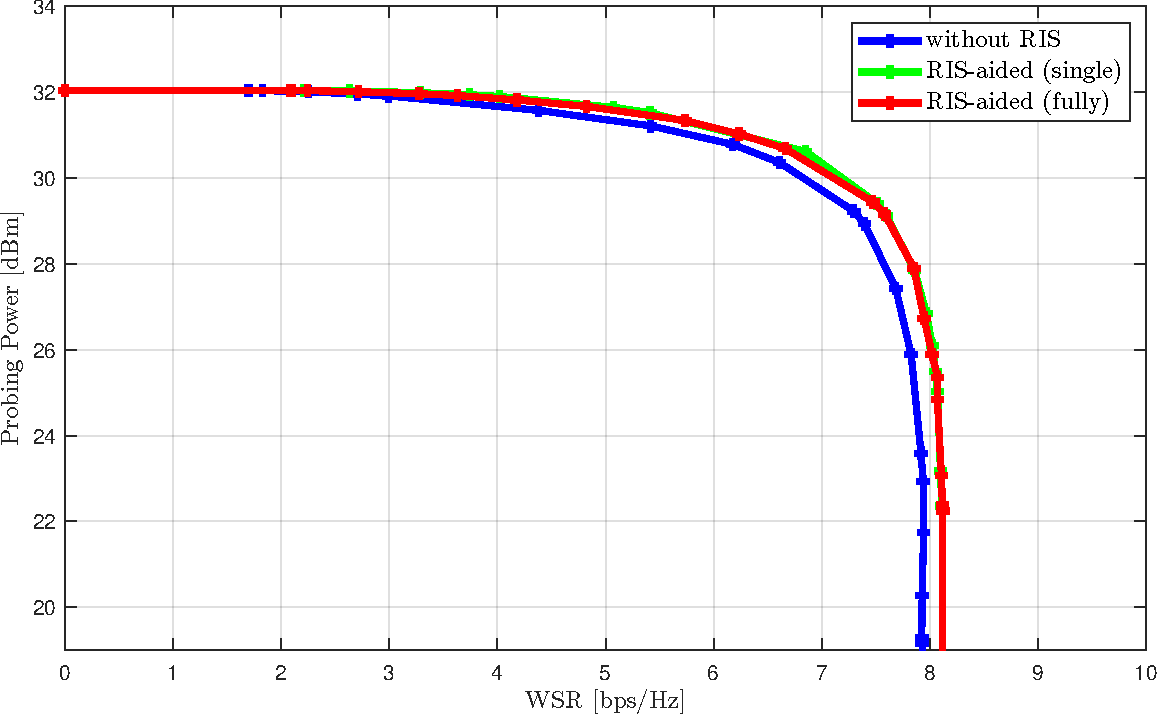
\includegraphics[width=0.475\textwidth]{tradeoff_single_fully_d.pdf}
        \label{fig:tradeoff_single_fully_d}
    }
    \caption{Tradeoff between probing power at target and WSR}
    \label{fig:tradeoff_single_fully}
\end{figure}

In Figure \ref{fig:tradeoff_single_fully_a}, it is obvious that we must decrease the probing power to increase 
the WSR and vice versa, which is a tradeoff. It is also clear that the RIS shows advantages 
compared with DFRC without RIS. 

For separated deployment, when the BS-RIS and RIS-user channels are Rayleigh channel (shown in Figure \ref{fig:tradeoff_single_fully_a}), 
the fully connected RIS performs best, which has a $6.0$bps/Hz upper bound of WSR. The single connected RIS is capable of 
achieving $5.8$bps/Hz upper bound of WSR, which is $0.20$bps/Hz higher than that achieved in the baseline. Figure \ref{fig:tradeoff_single_fully_b} 
shows that case where the channel is LOS dominated. One can visualize that the fully connected and single connected RIS has the same 
performance, which further validates the result in Section \ref{sec:beampattern_compare}.

Figure \ref{fig:tradeoff_single_fully_c} and \ref{fig:tradeoff_single_fully_d} show that the fully connected RIS only outperforms single connected RIS in Rayleigh channel for 
shared deployment, which is the same as separated deployment. However, the gain from RIS is smaller than that in separated deployment,
which is $0.15$bps/Hz and $0.27$bps/Hz for single connected and fully connected RIS in Rayleigh channel, respectively.

Although the RIS can increase the WSR upper bound, the 
probing power upper bounds are all $29$dBm in separated deployment and $32$dBm in shared deployment. 
The reason is that the probing power upper bound is determined by the capability of BS, which is the same when there is RIS or not.
There is a $3$dB gain of probing power upper bound for shared deployment over separated deployment.

We now evaluate the performance of DFRC aided by single connected RIS in LOS-dominated Rician channel with various numbers of reflecting elements. In Figure \ref{fig:tradeoff_reflecting_element}, we can see 
that the DFRC systems have the larger achievable region and higher WSR upper bounds as the increase of reflecting elements. The RIS 
with 100 elements is capable of improving the WSR by $0.82$bps/Hz in separated deployment and $0.58$bps/Hz in shared deployment. 
\begin{figure}[h]
    \centering
    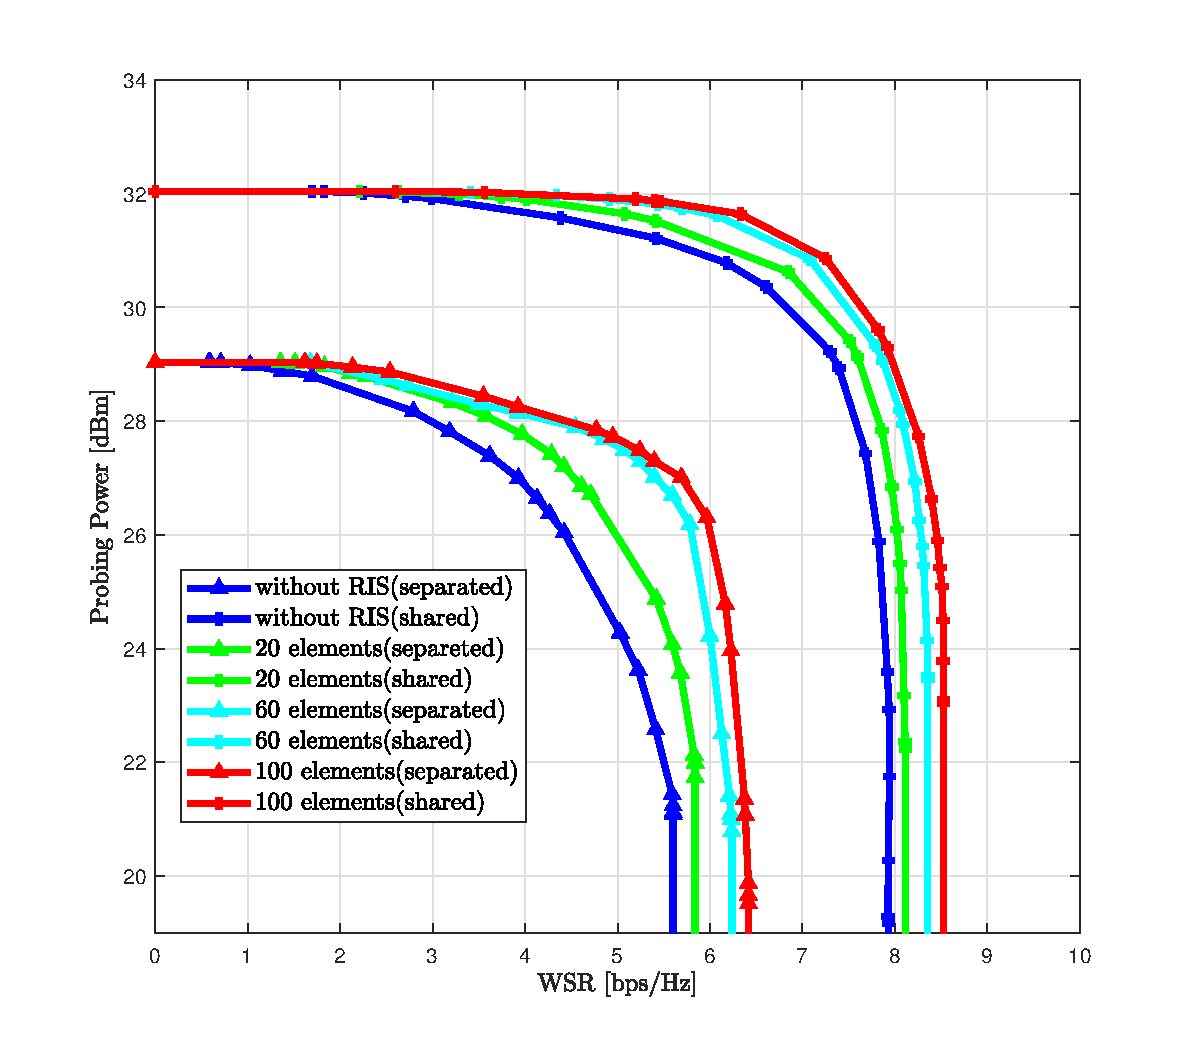
\includegraphics[width=1.0\textwidth]{tradeoff_reflecting_element.pdf}
    \caption{Effect of the number of reflecting elements on tradeoff in Rayleigh channels}
    \label{fig:tradeoff_reflecting_element}
\end{figure}